% !TeX program = lualatex

\documentclass[aspectratio=169,12pt,t]{beamer}
\usepackage[backend=biber,style=gb7714,gbpub=false]{biblatex}
\usepackage[fontset=none,scheme=plain]{ctex}
\usepackage{booktabs}
\usepackage{graphicx}
\usepackage{tabularx}

\usefonttheme{serif}
\setbeamertemplate{navigation symbols}{}
\setbeamertemplate{footline}[frame number]
\setbeamercolor{frametitle}{fg=black!80}
\setbeamerfont{frametitle}{size=\Large}

\setmainfont[Path=fonts/, BoldFont=*-Bold, UprightFont=*-regular, ItalicFont=*-It]{MinionPro}
% BabelStoneHan-merged.ttf 由 make font 生成：Basic、Extra、PUA 三字型按文中用字子集化後合併，
% 並以 liga 將 pua-ids.csv 所列 IDS 替換爲對應字形
\setCJKmainfont[Path=fonts/]{BabelStoneHan-merged.ttf}
% Add BSH PUA to JAchar
\ltjdefcharrange{6}{"E000-"F8FF}

\renewcommand{\bibfont}{\scriptsize}
\addbibresource{main.bib}

% 五行色標（依五色：木青、火赤、土黃、金白；金改用深金黃以利投影辨識，水改用藍以免與正文混淆）
\definecolor{wxmu}{RGB}{20,130,60}
\definecolor{wxhuo}{RGB}{200,30,30}
\definecolor{wxtu}{RGB}{128,128,77}
\definecolor{wxjin}{RGB}{205,150,0}
\definecolor{wxshui}{RGB}{25,75,185}
\newcommand{\Mu}{\textcolor{wxmu}{木}}
\newcommand{\Huo}{\textcolor{wxhuo}{火}}
\newcommand{\Tu}{\textcolor{wxtu}{土}}
\newcommand{\Jin}{\textcolor{wxjin}{金}}
\newcommand{\Shui}{\textcolor{wxshui}{水}}
% 五行字著色
\newcommand{\cmu}[1]{\textcolor{wxmu}{#1}}
\newcommand{\chuo}[1]{\textcolor{wxhuo}{#1}}
\newcommand{\ctu}[1]{\textcolor{wxtu}{#1}}
\newcommand{\cjin}[1]{\textcolor{wxjin}{#1}}
\newcommand{\cshui}[1]{\textcolor{wxshui}{#1}}

% 五行字注音：\wxpy{字} 於字上標拼音（每頁首次出現者，由 tools/add-ruby.py 標注）
% Minion Pro 缺第三聲字母（ǎ ǐ ǒ ǔ ǚ），拼音改用 EB Garamond
\newfontfamily\pinyinfont{EBGaramond-Regular.otf}
\makeatletter
\newcommand{\wxdefpy}[2]{\@namedef{wxpy@#1}{#2}}
% 拼音寬於字時加寬字框，避免與鄰字重疊；拼音計入行高，避免壓到上一行
\newcommand{\wxpy}[1]{\leavevmode\begingroup
  \setbox\z@\hbox{#1}%
  \setbox\tw@\hbox{\fontsize{\dimexpr0.6\dimexpr\f@size pt\relax\relax}{0pt}\selectfont
  \pinyinfont\@nameuse{wxpy@#1}}%
  \dimen@\wd\tw@ \advance\dimen@ 0.1em
  \ifdim\dimen@<\wd\z@ \dimen@\wd\z@ \fi
  \hbox{\rlap{\raise1em\hbox to\dimen@{\hss\box\tw@\hss}}%
  \hbox to\dimen@{\hss\box\z@\hss}}%
\endgroup}
\makeatother
% 拼音表：由 tools/add-ruby.py 依 Unihan 生成，只收文中用到之字。
% 表中已有之讀音不會被覆蓋，可手動修改或補入 Unihan 無讀音之字。
% BEGIN pinyin map
\wxdefpy{⿰口⿸户禾}{qú}
\wxdefpy{⿰木泴}{tà}
\wxdefpy{⿰氵翥}{zhù}
\wxdefpy{⿰音金}{[yīn]}
\wxdefpy{⿱金坐}{[cuò]}
\wxdefpy{⿺是火}{tǐ}
\wxdefpy{㐖}{xié}
\wxdefpy{㮅}{zhuī}
\wxdefpy{㷑}{yān}
\wxdefpy{㷤}{hù}
\wxdefpy{㾀}{qiè}
\wxdefpy{㾣}{qīn}
\wxdefpy{䐍}{chù}
\wxdefpy{䕸}{jiē}
\wxdefpy{䚜}{bī}
\wxdefpy{䚡}{sāi}
\wxdefpy{䞒}{dòng}
\wxdefpy{䞢}{zuó}
\wxdefpy{䡜}{lù}
\wxdefpy{䦯}{zhì}
\wxdefpy{䫦}{gé}
\wxdefpy{䮔}{zuī}
\wxdefpy{䵠}{dí}
\wxdefpy{休}{xiū}
\wxdefpy{侎}{mǐ}
\wxdefpy{光}{guāng}
\wxdefpy{剭}{wū}
\wxdefpy{勤}{qín}
\wxdefpy{去}{qù}
\wxdefpy{吉}{jí}
\wxdefpy{吙}{huō}
\wxdefpy{咣}{guāng}
\wxdefpy{唫}{jìn}
\wxdefpy{噤}{jìn}
\wxdefpy{土}{tǔ}
\wxdefpy{均}{jūn}
\wxdefpy{坖}{jì}
\wxdefpy{基}{jī}
\wxdefpy{堇}{jǐn}
\wxdefpy{堯}{yáo}
\wxdefpy{塣}{zhèng}
\wxdefpy{宷}{shěn}
\wxdefpy{嵤}{róng}
\wxdefpy{嶔}{qīn}
\wxdefpy{廞}{xīn}
\wxdefpy{憆}{chēng}
\wxdefpy{掛}{guà}
\wxdefpy{擁}{yōng}
\wxdefpy{斛}{hú}
\wxdefpy{木}{mù}
\wxdefpy{杰}{jié}
\wxdefpy{校}{xiào}
\wxdefpy{桂}{guì}
\wxdefpy{棡}{gāng}
\wxdefpy{棣}{dì}
\wxdefpy{榖}{gǔ}
\wxdefpy{榦}{gàn}
\wxdefpy{榮}{róng}
\wxdefpy{樉}{shuǎng}
\wxdefpy{樘}{táng}
\wxdefpy{標}{biāo}
\wxdefpy{橚}{sù}
\wxdefpy{檗}{bò}
\wxdefpy{檢}{jiǎn}
\wxdefpy{檭}{yín}
\wxdefpy{水}{shuǐ}
\wxdefpy{沀}{xù}
\wxdefpy{洛}{luò}
\wxdefpy{深}{shēn}
\wxdefpy{渠}{qú}
\wxdefpy{澃}{jiǒng}
\wxdefpy{火}{huǒ}
\wxdefpy{灮}{guāng}
\wxdefpy{炅}{jiǒng}
\wxdefpy{焋}{zhuàng}
\wxdefpy{熜}{cōng}
\wxdefpy{熲}{jiǒng}
\wxdefpy{熾}{chì}
\wxdefpy{理}{lǐ}
\wxdefpy{琱}{diāo}
\wxdefpy{眰}{diè}
\wxdefpy{碆}{bō}
\wxdefpy{禾}{hé}
\wxdefpy{穝}{zuō}
\wxdefpy{米}{mǐ}
\wxdefpy{糓}{gǔ}
\wxdefpy{腫}{zhǒng}
\wxdefpy{至}{zhì}
\wxdefpy{臵}{gé}
\wxdefpy{莎}{shā}
\wxdefpy{萩}{qiū}
\wxdefpy{螼}{qǐn}
\wxdefpy{衢}{qú}
\wxdefpy{覢}{shǎn}
\wxdefpy{角}{jiǎo}
\wxdefpy{觤}{guǐ}
\wxdefpy{訸}{hé}
\wxdefpy{詸}{mí}
\wxdefpy{謹}{jǐn}
\wxdefpy{賧}{tàn}
\wxdefpy{赤}{chì}
\wxdefpy{赮}{xiá}
\wxdefpy{走}{zǒu}
\wxdefpy{跿}{tú}
\wxdefpy{踏}{tá}
\wxdefpy{郮}{zhōu}
\wxdefpy{里}{lǐ}
\wxdefpy{量}{liàng}
\wxdefpy{金}{jīn}
\wxdefpy{鈞}{jūn}
\wxdefpy{鈺}{yù}
\wxdefpy{銜}{xián}
\wxdefpy{錐}{zhuī}
\wxdefpy{錖}{dú}
\wxdefpy{鎮}{zhèn}
\wxdefpy{隹}{zhuī}
\wxdefpy{雀}{què}
\wxdefpy{雋}{juàn}
\wxdefpy{頮}{huì}
\wxdefpy{騇}{shè}
\wxdefpy{魚}{yú}
\wxdefpy{魩}{mò}
\wxdefpy{鰾}{biào}
\wxdefpy{鱕}{fān}
\wxdefpy{黑}{hēi}
\wxdefpy{點}{diǎn}
\wxdefpy{黲}{cǎn}
\wxdefpy{𠒝}{bǐng}
\wxdefpy{𠟍}{chōng}
\wxdefpy{𠮷}{jí}
\wxdefpy{𠳊}{hē}
\wxdefpy{𡈾}{yì}
\wxdefpy{𡩁}{qīn}
\wxdefpy{𡸱}{lù}
\wxdefpy{𣹇}{kè}
\wxdefpy{𣹬}{hú}
\wxdefpy{𤋜}{zhào}
\wxdefpy{𤠿}{qiān}
\wxdefpy{𤦮}{zhì}
\wxdefpy{𥄳}{tà}
\wxdefpy{𥪢}{lóng}
\wxdefpy{𦧤}{tiè}
\wxdefpy{𧗱}{shù}
\wxdefpy{𧩼}{chì}
\wxdefpy{𧹝}{tóng}
\wxdefpy{𧽧}{chù}
\wxdefpy{𨥷}{lìng}
\wxdefpy{𨼪}{chǔ}
\wxdefpy{𩀈}{xuān}
\wxdefpy{𩀡}{nán}
\wxdefpy{𩁜}{lěi}
\wxdefpy{𩅠}{nàn}
\wxdefpy{𩉍}{jiǎn}
\wxdefpy{𩒪}{zhèn}
\wxdefpy{𩵛}{biē}
\wxdefpy{𩶀}{[yá]}
\wxdefpy{𩿹}{qiè}
\wxdefpy{𪇼}{nán}
\wxdefpy{𪑙}{jīn}
\wxdefpy{𪒯}{qín}
\wxdefpy{𪔄}{zī}
\wxdefpy{𪢍}{jié}
\wxdefpy{𰍠}{níng}
\wxdefpy{𰝙}{ān}
\wxdefpy{𰟆}{jí}
\wxdefpy{𰨘}{wàn}
\wxdefpy{𰼪}{mú}
\wxdefpy{⿱頂土}{diān}
\wxdefpy{⿱坴火}{chì}
\wxdefpy{𣲎}{yǐn}
\wxdefpy{鑫}{xīn}
\wxdefpy{㵗}{píng}
% END pinyin map
\newcommand{\src}[1]{{\footnotesize\color{black!55}#1}}
\setbeamercolor{description item}{fg=black!70}

% 英譯：\en 另起一行小字；\entext 行內小字；\bi{中}{英} 表頭中英雙行；標題英譯用 frame 副標題
\newcommand{\entext}[1]{{\scriptsize\color{black!60}#1}}
\newcommand{\en}[1]{\par{\parskip=0pt\scriptsize\color{black!60}#1\par}}
\newcommand{\bi}[2]{\begin{tabular}[b]{@{}c@{}}#1\\[-0.3ex]\entext{#2}\end{tabular}}
\setbeamerfont{framesubtitle}{size=\footnotesize}
\setbeamercolor{framesubtitle}{fg=black!55}

% 引用上標改灰色，減少視覺干擾
\definecolor{citegray}{gray}{0.55}
\AtBeginDocument{%
  \renewcommand*\mkbibsuperbracket[1]{%
\mkbibsuperscript{\color{citegray}\mkbibleftborder{#1}\mkbibrightborder}}}

% tabularx 置中欄
\newcolumntype{Y}{>{\centering\arraybackslash}X}

% 五行用例表：左欄部件與例字，右欄人名用例
\newenvironment{wxtab}
{\footnotesize\renewcommand{\arraystretch}{1.15}%
\tabularx{\textwidth}{@{}>{\raggedright\arraybackslash}p{11em}>{\raggedright\arraybackslash}X@{}}\toprule}
{\bottomrule\endtabularx\par\medskip}
\newcommand{\wxrow}[3]{\leavevmode{\color{black!65}#1}\par\smallskip{\normalsize #2} & #3 \\ \addlinespace[0.5em]}

\title{明代宗室命名規則中的五行用字}
\subtitle{Five-Phase Characters in the Naming of the Ming Imperial Clan}
\author{Huáng Jùnliàng (黄俊亮)}
\date{\today}

\begin{document}

\begin{frame}[c]
  \titlepage
\end{frame}

\begin{frame}{自我介紹}{Self-introduction}
  \bi{黄俊亮}{Huáng Jùnliàng}\\
  \begin{itemize}
    \item 自2021年起擔任IRG個人專家，專注審閱古籍用字，幫助維護ORT系統
    \en{IRG Individual Expert since 2021, focused on reviewing rare characters in historical Chinese texts and helping maintain the online review tool (ORT)}
    \item BabelStone Han字體維護者，該字體由已故IRG專家魏安創建
    \en{Maintainer of BabelStone Han font, created by the late IRG expert Andrew West}
    \item Babel團隊核心成員。Babel是一個將未來的JavaScript編譯為當前JavaScript的開源項目
    \en{Core member of the Babel team, an open source project to compile future JavaScript to current JavaScript}
  \end{itemize}
\end{frame}

% ---------------------------------------------------------------------------
\begin{frame}{緣起：朱元璋擬定「二十字」字輩}{Origins: Zhu Yuanzhang's twenty-character generation poems}
  \begin{block}{朱元璋《皇明祖訓》\entext{\quad Zhu Yuanzhang, \emph{Ancestral Instructions}}}
    凡東宮親王位下，各擬名二十字，日後生子及孫，即以上聞，付宗人府。所立𩀱名，每一世𲹨一字，以為上字。其下一字，臨時隨意選擇，以為𩀱名，編入玉牒。至二十世後照例續添，永為定式。\cite[20]{皇明祖訓}
    \en{For the Heir Apparent's line and each prince's line, twenty name characters are drafted; sons and grandsons are reported to the throne and the Imperial Clan Court. Each generation takes the next character as the first of its two-character names; the second is chosen freely at the time. Names go into the Jade Register; after twenty generations more are added. This is a permanent rule.}
  \end{block}
  \vspace{0.2em}
  \begin{columns}[T]
    \column{0.5\textwidth}
    \textbf{東宮位下}\entext{\quad Line of the Heir Apparent}\\
    允文遵祖訓，欽武大君勝。\\
    順道宜逢吉，師良善用晟。
    \column{0.5\textwidth}
    \textbf{燕王位下}（成祖以後帝系）\\
    \entext{Line of the Prince of Yan (imperial line from Chengzu on)}\\
    高瞻祁見祐，厚載翊常由。\\
    慈和怡伯仲，簡靖迪先猷。
  \end{columns}
  \vspace{0.2em}
  \begin{itemize}
    \item 雙名之\textbf{上字}：依字輩，一世一字\quad\entext{First character: from the poem, one per generation}
    \item 雙名之\textbf{下字}：「臨時隨意選擇」——後世實務上不隨意\quad\entext{Second: not really ``free''}
  \end{itemize}
\end{frame}

% ---------------------------------------------------------------------------
\begin{frame}{下字規則：五行相生}{The second character: the generating cycle of the Five Phases}
  \begin{block}{何喬遠《名山藏》\entext{\quad He Qiaoyuan, \emph{Mingshan cang}}}
    命名以五行相生一字爲偏傍以綴之。其後宗室繁多，五行偏傍已窮，皆翰林雜製定音而字義無取焉\cite[35:1a]{名山藏}。
    \en{Names were completed with a character whose radical is one of the Five Phases, in generating order. Later the clan grew so large that the Five-Phase radicals were exhausted, and Hanlin academicians made up characters with a fixed reading but no meaning.}
  \end{block}
  \vspace{1em}
  \begin{center}
    \Mu{} → \Huo{} → \Tu{} → \Jin{} → \Shui{} → \Mu{} → ……
    \en{Wood → Fire → Earth → Metal → Water → Wood → …}
  \end{center}
  \vspace{0.5em}
  太祖諸子之名皆從\Mu（\cmu{\wxpy{標}、\wxpy{樉}、\wxpy{棡}、\wxpy{棣}、\wxpy{橚}}……），其下一世從\Huo，依次相生。
  \en{The names of Taizu's sons all take Wood; the next generation takes Fire, and so on through the cycle.}
\end{frame}

% ---------------------------------------------------------------------------
\begin{frame}{下字規則：帝系實例}{The second character: the imperial line}
  \textbf{燕王位下}（成祖以後帝系）\entext{\quad Line of the Prince of Yan (imperial line from Chengzu on)}\\
    高瞻祁見祐，厚載翊常由。慈和怡伯仲，簡靖迪先猷。
  \centering
  \begin{tabularx}{\linewidth}{c c c X @{\hspace{3em}} c c X}
    \toprule
    \bi{五行}{Phase} & \bi{字輩}{Gen.} & \bi{下字}{2nd} & \bi{廟號}{Temple name} & \bi{字輩}{Gen.} & \bi{下字}{2nd} & \bi{廟號}{Temple name} \\
    \midrule
     \Mu   & —  & \cmu{\wxpy{棣}} & 成祖 & \multicolumn{3}{c}{（接續左半）\entext{continued from left}} \\
     \Huo  & 高 & \chuo{\wxpy{熾}} & 仁宗 & 厚  & \chuo{\wxpy{𤋜}}\cite[61]{明孝宗實錄}、\chuo{ \wxpy{熜}} & 武宗、世宗 \\
    \Tu   & 瞻 &  \ctu{\wxpy{基}} & 宣宗 & 載  & \ctu{\wxpy{坖}}\cite[200]{明世宗實錄} & 穆宗 \\
    \Jin  & 祁 &  \cjin{\wxpy{鎮}}、\cjin{\wxpy{鈺}} & 英宗、代宗 & 翊  & \cjin{\wxpy{鈞}} & 神宗 \\
    \Shui & 見 &  \cshui{\wxpy{深}} & 憲宗 & 常 & \cshui{\wxpy{洛}} & 光宗 \\
    \Mu   & 祐 & \cmu{\wxpy{樘}} & 孝宗 & 由 & \cmu{\wxpy{校}、\wxpy{檢}} & 熹宗、思宗 \\
    \bottomrule
  \end{tabularx}
\end{frame}

% ---------------------------------------------------------------------------
\begin{frame}{各藩字輩與五行對應：太祖以下}{Generation characters and phases by princely house: Taizu's sons}
  \centering
  \scriptsize
  \setlength{\tabcolsep}{1.9pt}
  \renewcommand{\arraystretch}{1.05}
  \begin{tabularx}{\linewidth}{|c|c|*{18}{Y|}}
    \hline
    世 & 五行 & 帝系 & 秦 & 晉 & 周 & 楚 & 齊 & 魯 & 蜀 & 代 & 肅 & 遼 & 慶 & 寧 & 岷 & 韓 & 瀋 & 唐 & 伊 \\
    \hline
    封地 &  & & 西安 & 太原 & 開封 & 武昌 & 南京 & 兗州 & 成都 & 大同 & 臨洮 & 荊州 & 寧夏 & 南昌 & 武岡 & 平涼 & 潞州 & 南陽 & 洛陽 \\
    \hline\hline
    2 & \Huo & 高 & 尚 & 濟 & 有 & 孟 & 賢 & 肇 & 悅 & 遜 & 贍 & 貴 & 秩 & 磐 & 徽 & 沖 & 佶 & 瓊 & 顒 \\ \hline
    3 & \Tu & 瞻 & 志 & 美 & 子 & 季 & 能 & 泰 & 友 & 仕 & 祿 & 豪 & 邃 & 奠 & 音 & 範 & 幼 & 芝 & 勉 \\ \hline
    4 & \Jin & 祁 & 公 & 鍾 & 同 & 均 & 長 & 陽 & 申 & 成 & 貢 & 恩 & 寘 & 覲 & 膺 & 徵 & 詮 & 彌 & 諟 \\ \hline
    5 & \Shui & 見 & 誠 & 奇 & 安 & 榮 & 可 & 當 & 賓 & 聰 & 真 & 寵 & 台 & 宸 & 彦 & 偕 & 勛 & 宇 & 訏 \\ \hline
    6 & \Mu & 祐 & 秉 & 表 & 睦 & 顯 & 慶 & 健 & 讓 & 俊 & 弼 & 致 & 鼒 & 拱 & 譽 & 旭 & 胤 & 宙 & 典 \\ \hline
    7 & \Huo & 厚 & 惟 & 知 & 勤 & 英 & 睿 & 觀 & 承 & 充 & 縉 & 憲 & 倪 & 多 & 定 & 融 & 恬 & 碩 & 褒 \\ \hline
    8 & \Tu & 載 & 懷 & 新 & 朝 & 華 & 知 & 頤 & 宣 & 廷 & 紳 & 術 & 伸 & 謀 & 幹 & 謨 & 珵 & 器 & 珂 \\ \hline
    9 & \Jin & 翊 & 敬 & 慎 & 在 & 蘊 & 實 & 壽 & 奉 & 鼐 & 識 & 儼 & 帥 & 統 & 企 & 朗 & 效 & 聿 & 采 \\ \hline
    10 & \Shui & 常 & 誼 & 敏 & 肅 & 盛 & 堪 & 以 & 至 & 鼎 & 烈 & 尊 & 倬 & 議 & 禋 & 璟 & 迥 & 琳 & 鳳 \\ \hline
    11 & \Mu & 由 & 存 & 求 & 恭 & 容 & 宗 & 弘 & 平 & 彝 & 忠 & 儒 & 奇 & 中 & 雍 & 逵 & 瑝 & 琚 & 琛 \\ \hline
    12 & \Huo & 慈 & 輔 & 審 & 紹 & 宏 & 養 & 振 & 懋 & 傳 & 曦 & 雲 & 适 & 總 & 崇 & 亶 & 湜 & 啟 & 應 \\ \hline
    13 & \Tu & 和 & 嗣 & 心 & 倫 & 才 & 性 & 舉 & 進 & 貽 & 暉 & 仍 & 完 & 添 & 理 & 韶 & 源 & 齡 & 疇 \\ \hline
  \end{tabularx}

  \en{世 generation; 五行 phase; 帝系 imperial line; 封地 fief}
  \begin{itemize}
    \item 太祖諸子爲第1世。各藩字輩不同，但同一世的下字五行全國一致。
      \en{Taizu's sons are generation 1. Each house has its own poem, but within a generation the phase of the second character is the same everywhere.}
  \end{itemize}
\end{frame}

% ---------------------------------------------------------------------------
\begin{frame}{各藩字輩與五行對應：太祖以下（續）}{Generation characters by princely house: notes on the table}
  \begin{itemize}
    \item 齊王封地青州，後廢爲庶人，子孫皆居應天府（南京）。
      \en{The Prince of Qi was enfeoffed at Qingzhou; after he was made a commoner, his descendants lived in Yingtian (Nanjing).}
    \item 晉藩第7世「知」與齊藩第8世「知」同字。實務上齊藩「知」亦常書作「智」。
      \en{Jin gen.~7 and Qi gen.~8 both use 知; in practice Qi's 知 is often written 智.}
    \item 晉藩第5世「奇」與慶藩第11世「奇」同字。未見慶藩第11世宗室命名實例。
      \en{Jin gen.~5 and Qing gen.~11 both use 奇; no named member of Qing gen.~11 is attested.}
  \end{itemize}
\end{frame}

% ---------------------------------------------------------------------------
\begin{frame}{各藩字輩與五行對應：成祖以下}{Generation characters and phases by princely house: Chengzu's descendants}
  \centering
  \scriptsize
  \setlength{\tabcolsep}{1.9pt}
  \renewcommand{\arraystretch}{1.05}
  \begin{tabularx}{\linewidth}{|c|c|*{16}{Y|}}
    \hline
    世 & 五行 & 帝系 & 趙 & 鄭 & 襄 & 荊 & 淮 & 德 & 崇 & 吉 & 徽 & 益 & 衡 & 榮 & 潞 & 福 & 桂 \\
    \hline
    封地 & & & 彰德 & 懷慶 & 襄陽 & 蘄州 & 饒州 & 濟南 & 汝寧 & 長沙 & 鈞州 & 建昌 & 青州 & 常德 & 衛輝 & 洛陽 & 衡州 \\
    \hline\hline
    2 & \Huo & \multicolumn{2}{c|}{高} & \multicolumn{4}{c|}{} & \multicolumn{4}{c|}{} & \multicolumn{3}{c|}{} & & \multicolumn{2}{c|}{} \\ \hline
    3 & \Tu & \multicolumn{2}{c|}{瞻} & \multicolumn{4}{c|}{瞻} & \multicolumn{4}{c|}{} & \multicolumn{3}{c|}{} & & \multicolumn{2}{c|}{} \\ \hline
    4 & \Jin & \multicolumn{2}{c|}{祁} & \multicolumn{4}{c|}{祁} & \multicolumn{4}{c|}{} & \multicolumn{3}{c|}{} & & \multicolumn{2}{c|}{} \\ \hline
    5 & \Shui & \multicolumn{2}{c|}{見} & \multicolumn{4}{c|}{見} & \multicolumn{4}{c|}{見} & \multicolumn{3}{c|}{} & & \multicolumn{2}{c|}{} \\ \hline
    6 & \Mu & \multicolumn{2}{c|}{祐} & \multicolumn{4}{c|}{祐} & \multicolumn{4}{c|}{祐} & \multicolumn{3}{c|}{祐} & & \multicolumn{2}{c|}{} \\ \hline
    7 & \Huo & \multicolumn{2}{c|}{厚} & \multicolumn{4}{c|}{厚} & \multicolumn{4}{c|}{厚} & \multicolumn{3}{c|}{厚} & & \multicolumn{2}{c|}{} \\ \hline
    8 & \Tu & \multicolumn{2}{c|}{載} & \multicolumn{4}{c|}{載} & \multicolumn{4}{c|}{載} & \multicolumn{3}{c|}{載} & & \multicolumn{2}{c|}{} \\ \hline
    9 & \Jin & \multicolumn{2}{c|}{翊} & \multicolumn{4}{c|}{翊} & \multicolumn{4}{c|}{翊} & \multicolumn{3}{c|}{翊} & 翊 & \multicolumn{2}{c|}{} \\ \hline
    10 & \Shui & \multicolumn{2}{c|}{常} & \multicolumn{4}{c|}{常} & \multicolumn{4}{c|}{常} & \multicolumn{3}{c|}{常} & 常 & \multicolumn{2}{c|}{常} \\ \hline
    11 & \Mu & \multicolumn{2}{c|}{由} & \multicolumn{4}{c|}{由} & \multicolumn{4}{c|}{由} & \multicolumn{3}{c|}{由} & 由 & \multicolumn{2}{c|}{由} \\ \hline
    12 & \Huo & \multicolumn{2}{c|}{慈} & \multicolumn{4}{c|}{慈} & \multicolumn{4}{c|}{慈} & \multicolumn{3}{c|}{慈} & 慈 & \multicolumn{2}{c|}{慈} \\ \hline
    13 & \Tu & \multicolumn{2}{c|}{和} & \multicolumn{4}{c|}{和} & \multicolumn{4}{c|}{和} & \multicolumn{3}{c|}{和} & 和 & \multicolumn{2}{c|}{和} \\ \hline
  \end{tabularx}
  \vspace{0.5em}
  \begin{itemize}
  \item 成祖以下諸藩沿用燕王位下字輩，故與帝系同字；空格表示該藩尚未分封。
    \en{Houses descended from Chengzu use the Yan poem, so they share the imperial line's characters; a blank cell means the house did not yet exist.}
  \item 以上二表僅羅列2--13世：明亡時宗室約傳至第13世。
    \en{Both tables cover generations 2--13 only: when the Ming fell, the clan had reached about generation 13.}
  \end{itemize}
\end{frame}

% ---------------------------------------------------------------------------
\begin{frame}{問題：「五行偏傍已窮」之後怎麼辦？}{The problem: what happens once ``the Five-Phase radicals are exhausted''?}
  \begin{itemize}
    \item 明中葉以後宗室人口激增，同一藩同一世人數眾多
      \en{From the mid-Ming on the clan grew rapidly; each generation of a house had many members}
    \item 名字不得重複，帶\Mu\Huo\Tu\Jin\Shui{}部首的常用字很快用盡
      \en{Names could not repeat, so common characters with a Wood, Fire, Earth, Metal or Water radical soon ran out}
    \item 結果：大量罕用字、新造字進入宗室名字
      \en{Result: many rare and newly coined characters entered clan names}
      \begin{itemize}
        \item 不少字至今仍未編碼，或字形在後世文獻中被「校正」
          \en{Many are still not encoded, or their forms were ``corrected'' in later texts}
      \end{itemize}
  \end{itemize}
  \vspace{1em}
  \begin{alertblock}{觀察\entext{\quad Observation}}
    五行之判斷，不限於\textbf{部首}；凡字形中含有該行之\textbf{部件}，即可作該行字用。
    \en{A character's phase is not limited to its \textbf{radical}: any character whose form contains a phase's \textbf{component} can serve as a character of that phase.}
  \end{alertblock}
\end{frame}

% ---------------------------------------------------------------------------
\begin{frame}{\Mu{}行字（一）}{Wood characters (1)}
  \begin{wxtab}
    \wxrow{傳統木部}{\cmu{\wxpy{樘}\hspace{1em}\wxpy{檗}\hspace{1em}\wxpy{榖}\hspace{1em}\wxpy{㮅}\hspace{1em}\wxpy{⿰木泴}}}{孝宗朱祐\cmu{樘}\cite[141:5b]{明憲宗實錄}、周藩遂平端靖王朱睦\cmu{檗}\cite[6:5a]{萬曆開封府志}、韓藩褒城輔國將軍朱旭\cmu{榖}\cite[64]{明世宗實錄}、代藩山陰鎮國將軍朱俊\cmu{㮅}\cite[]{山陰榮靖王妃張氏壙誌文}、德藩清平鎮國將軍朱由\cmu{\mbox{⿰木泴}}\cite[]{明史德王府世系表訂誤}（未編碼\quad\entext{Unencoded}）}
    \wxrow{含木部件}{\cmu{\wxpy{𨼪}\hspace{1em}\wxpy{休}\hspace{1em}\wxpy{榦}\hspace{1em}\wxpy{𡩁}\hspace{1em}\wxpy{噤}\hspace{1em}\wxpy{𦧤}}}{周藩臨汝王朱睦\cmu{𨼪}\cite[395]{明神宗實錄}、楚藩崇陽王朱顯\cmu{休}\cite[19:3b]{明世宗實錄}、肅藩康裕王朱弼\cmu{榦}\cite[502:5b]{明世宗實錄}、代藩襄垣鎮國中尉朱俊\cmu{𡩁}\cite[三集:7:37a]{續垂棘編}、代藩襄垣奉國將軍朱俊\cmu{噤}\cite{朱俊噤普救寺塔詩碣}、寧藩石城奉國中尉朱中\cmu{𦧤}\cite[2:93a]{盱眙朱氏八支宗譜}}
  \end{wxtab}
\end{frame}

% ---------------------------------------------------------------------------
\begin{frame}{\Mu{}行字（二）}{Wood characters (2)}
  \begin{wxtab}
    \wxrow{含米部件}{\cmu{\wxpy{侎}\hspace{1em}\wxpy{𧗱}\hspace{1em}\wxpy{宷}\hspace{1em}\wxpy{糓}\hspace{1em}\wxpy{詸}}}{德藩紀城王朱由\cmu{侎}\cite[482]{明神宗實錄}、寧藩石城奉國中尉朱中\cmu{𧗱}\cite[2:94a]{盱眙朱氏八支宗譜}、寧藩石城奉國中尉朱中\cmu{宷}\cite[2:83b]{盱眙朱氏八支宗譜}、遼藩巴東奉國中尉朱致\cmu{糓}\cite[2:34b]{萬曆荊州志}、代藩隰川鎮國中尉朱俊\cmu{詸}\cite{皇明隰川王府奉國將軍慎齋公墓誌銘}}
    \wxrow{含禾部件}{\cmu{\wxpy{訸}\hspace{1em}\wxpy{穝}\hspace{1em}\wxpy{萩}\hspace{1em}\wxpy{⿰口⿸户禾}}}{周藩封丘肅安王朱睦\cmu{訸}\cite[421:6b]{明世宗實錄}、韓藩樂平奉國將軍朱旭\cmu{穝}\cite[7:39b]{趙浚谷文集}、
      %https://commons.wikimedia.org/wiki/File:NLC892-GBZX0301010963-254568_%E8%B6%99%E6%B5%9A%E8%B0%B7%E6%96%87%E9%9B%86_%E5%8D%81%E5%8D%B7_%E7%AC%AC7%E5%86%8A.pdf
    益藩宗室朱由\cmu{萩}\cite[1:3a]{澹寧居文集}、寧藩石城奉國中尉朱中\cmu{\mbox{⿰口⿸户禾}}\cite[2:93b]{盱眙朱氏八支宗譜}（未編碼\quad\entext{Unencoded}）}
  \end{wxtab}
  \src{「米」「禾」均含「木」形，可作木行字。}\quad\entext{米 and 禾 both contain the shape of 木, so they count as Wood.}
\end{frame}

% ---------------------------------------------------------------------------
\begin{frame}{\Huo{}行字（一）}{Fire characters (1)}
  \begin{wxtab}
    \wxrow{傳統火部}{\chuo{\wxpy{熾}\hspace{1em}\wxpy{炅}\hspace{1em}\wxpy{𰟆}\hspace{1em}\wxpy{㷑}\hspace{1em}\wxpy{㷤}\hspace{1em}\wxpy{⿱坴火}}}{仁宗朱高\chuo{熾}\cite[119]{明太祖實錄}、慶藩安塞宣靖王朱秩\chuo{炅}\cite[118]{明英宗實錄}、代藩饒陽王朱充\chuo{𰟆}\cite[338]{明世宗實錄}、荊王朱慈\chuo{㷑}\cite[87]{明熹宗實錄}、代藩襄垣革爵輔國中尉朱充\chuo{㷤}\cite[27]{明神宗實錄}、寧藩宜春庶人朱多\chuo{⿱坴火}\cite[3:21b]{萬曆江西省大志}（未編碼\quad\entext{Unencoded}）}
    \wxrow{含火部件}{\chuo{\wxpy{𡸱}\hspace{1em}\wxpy{熲}\hspace{1em}\wxpy{𩒪}\hspace{1em}\wxpy{吙}\hspace{1em}\wxpy{覢}\hspace{1em}\wxpy{賧}\hspace{1em}\wxpy{嵤}\hspace{1em}\wxpy{⿺是火}}}{韓敬王朱亶\chuo{𡸱}\cite[482]{明神宗實錄}、周藩遂平悼恭王朱有\chuo{熲}\cite[19]{明宣宗實錄}、德藩紀城王朱慈\chuo{𩒪}\cite{明史德王府世系表訂誤}、慶藩弘農宗室朱倪\chuo{吙}\cite[286]{明神宗實錄}、慶藩安化輔國中尉朱倪\chuo{覢}\cite[286]{明神宗實錄}、晉藩方山奉國將軍朱知\chuo{賧}\cite[347]{明世宗實錄}、遼藩遠安奉國中尉朱憲\chuo{嵤}\cite[2:23a]{萬曆荊州志}、代藩靈丘輔國中尉朱充\chuo{⿺是火}\cite[9:9b]{龍塢集}（未編碼\quad\entext{Unencoded}）}
    \wxrow{含光部件}{\chuo{\wxpy{灮}\hspace{1em}\wxpy{咣}\hspace{1em}\wxpy{𠒝}}}{周藩永寧靖僖王朱有\chuo{灮}\cite[11]{明太宗實錄}、晉藩陽曲王府朱知\chuo{咣}\cite[488]{明神宗實錄}、代藩輔國將軍朱充\chuo{𠒝}\cite[49]{明神宗實錄}}
  \end{wxtab}
  \src{「光」古作「灮」，上部即火。}\quad\entext{光 was anciently written 灮, whose upper part is 火.}
\end{frame}

% ---------------------------------------------------------------------------
\begin{frame}{\Huo{}行字（二）}{Fire characters (2)}
  \begin{wxtab}
    \wxrow{含魚部件}{\chuo{\wxpy{魩}\hspace{1em}\wxpy{鰾}\hspace{1em}\wxpy{𩶀}\hspace{1em}\wxpy{鱕}\hspace{1em}\wxpy{𩵛}}}{蜀藩慶符王朱承\chuo{魩}\cite[506]{明神宗實錄}、唐藩承休王朱碩\chuo{鰾}\cite[298]{明神宗實錄}、代藩懷仁輔國中尉朱充\chuo{𩶀}\cite[37]{明熹宗實錄}、寧藩樂安鎮國中尉朱多\chuo{鱕}\cite[3]{萬曆江西省大志}、遼藩宜城鎮國中尉朱憲\chuo{𩵛}\cite[2]{萬曆荊州志}}
    \wxrow{含黑部件}{\chuo{\wxpy{𪒯}\hspace{1em}\wxpy{點}\hspace{1em}\wxpy{黲}\hspace{1em}\wxpy{䵠}\hspace{1em}\wxpy{䕸}}}{周藩義陽王朱勤\chuo{𪒯}\cite[408]{明神宗實錄}、晉藩慶成鎮國中尉朱知\chuo{點}\cite[232]{明世宗實錄}、周藩輔國將軍朱勤\chuo{黲}\cite[49]{明神宗實錄}、寧藩瑞昌奉國將軍朱多\chuo{䵠}\cite[3]{萬曆江西省大志}、周藩鎮平輔國中尉朱勤\chuo{䕸}\cite[15:20a]{昭甫集}}
  \end{wxtab}
  \src{「魚」「黑」下部之「灬」即火。注音帶[]標記者爲有邊讀邊的擬音。}
  \entext{The 灬 at the bottom of 魚 and 黑 is 火. Readings in [\,] are guesses from the phonetic.}
\end{frame}

% ---------------------------------------------------------------------------
\begin{frame}{\Tu{}行字（一）}{Earth characters (1)}
  \begin{wxtab}
    \wxrow{傳統土部}{\ctu{\wxpy{坖}\hspace{1em}\wxpy{均}\hspace{1em}\wxpy{堯}\hspace{1em}\wxpy{𡈾}\hspace{1em}\wxpy{⿱頂土}}}{穆宗朱載\ctu{坖}\cite[200]{明世宗實錄}、秦懷王朱志\ctu{均}\cite[3上]{明仁宗實錄}、瀋定王朱珵\ctu{堯}\cite[461]{明世宗實錄}、秦藩永壽輔國中尉朱懷\ctu{𡈾}\cite{朱惟躞墓誌銘}、慶藩延川奉國將軍朱伸\ctu{⿱頂土}\cite[2:8a]{萬曆朔方新志}（未編碼\quad\entext{Unencoded}）}
    \wxrow{含土部件}{\ctu{\wxpy{掛}\hspace{1em}\wxpy{䮔}\hspace{1em}\wxpy{𤠿}\hspace{1em}\wxpy{䡜}\hspace{1em}\wxpy{憆}\hspace{1em}\wxpy{𪔄}}}{魯藩新蔡王朱頤\ctu{掛}\cite[561]{明神宗實錄}、周藩萊陽王朱朝\ctu{䮔}\cite[284]{明神宗實錄}、淮藩南康鎮國將軍朱載\ctu{𤠿}\cite[3:7a]{萬曆江西省大志}、淮藩德興輔國將軍朱載\ctu{䡜}\cite[3:8a]{萬曆江西省大志}、寧藩弋陽鎮國中尉朱謀\ctu{憆}\cite[3]{萬曆江西省大志}、寧藩瑞昌輔國中尉朱謀\ctu{𪔄}\cite[4:161a]{盱眙朱氏八支宗譜}}
    \wxrow{含隹部件}{\ctu{\wxpy{𩀈}\hspace{1em}\wxpy{𰨘}\hspace{1em}\wxpy{雋}\hspace{1em}\wxpy{雀}\hspace{1em}\wxpy{𩁜}\hspace{1em}\wxpy{擁}\hspace{1em}\wxpy{衢}\hspace{1em}\wxpy{𩀡}}}{慶藩鎮原王朱伸\ctu{𩀈}\cite[257]{明神宗實錄}、蜀藩汶川王朱宣\ctu{𰨘}\cite[2:18a]{萬曆四川總志47}、寧藩石城輔國中尉朱謀\ctu{雋}\cite[3]{萬曆江西省大志}、寧藩石城輔國中尉朱謀\ctu{雀}\cite[3]{萬曆江西省大志}、遼藩巴東奉國中尉朱術\ctu{𩁜}\cite[2:25b]{萬曆荊州志}、寧藩瑞昌鎮國中尉朱謀\ctu{擁}\cite[3]{萬曆江西省大志}、寧藩瑞昌鎮國中尉朱謀\ctu{衢}\cite[3]{萬曆江西省大志}、遼藩益陽輔國中尉朱術\ctu{𩀡}\cite[2]{萬曆荊州志}}
  \end{wxtab}
  \src{「隹」下部含「土」形。}\quad\entext{The lower part of 隹 contains the shape of 土.}
\end{frame}

% ---------------------------------------------------------------------------
\begin{frame}{\Tu{}行字（二）}{Earth characters (2)}
  \begin{wxtab}
    \wxrow{含去部件}{\ctu{\wxpy{𩿹}\hspace{1em}\wxpy{㾀}\hspace{1em}\wxpy{䫦}\hspace{1em}\wxpy{𠳊}}}{寧藩石城鎮國中尉朱謀\ctu{𩿹}\cite[3]{萬曆江西省大志}、寧藩建安宗室朱謀\ctu{㾀}\cite[3:103a]{萬曆江西省大志}、遼藩松滋奉國將軍朱術\ctu{䫦}\cite[2]{萬曆荊州志}、秦藩永壽奉國中尉朱懷\ctu{𠳊}\cite{朱惟煠墓誌}}
    \wxrow{含角部件}{\ctu{\wxpy{䚜}\hspace{1em}\wxpy{觤}\hspace{1em}\wxpy{䚡}\hspace{1em}\wxpy{斛}}}{寧藩宜春宗室朱謀\ctu{䚜}\cite[3]{萬曆江西省大志}、寧藩建安宗室朱謀\ctu{觤}\cite[3:103a]{萬曆江西省大志}、寧藩建安宗室朱謀\ctu{䚡}\cite[3:104a]{萬曆江西省大志}、秦藩永壽輔國中尉朱懷\ctu{斛}\cite[]{朱惟焎墓誌銘}}
    \wxrow{含至部件}{\ctu{\wxpy{眰}\hspace{1em}\wxpy{臵}\hspace{1em}\wxpy{𧩼}\hspace{1em}\wxpy{剭}\hspace{1em}\wxpy{䦯}}}{遼藩益陽輔國中尉朱術\ctu{眰}\cite[2]{萬曆荊州志}、寧藩石城鎮國中尉朱謀\ctu{臵}\cite[3]{萬曆江西省大志}、寧藩弋陽宗室朱謀\ctu{𧩼}\cite[3]{萬曆江西省大志}、寧藩瑞昌鎮國中尉朱謀\ctu{剭}\cite[3]{萬曆江西省大志}、寧藩宜春奉國中尉朱謀\ctu{䦯}\cite[3:34a]{萬曆江西省大志}}
    \wxrow{含里部件}{\ctu{\wxpy{理}\hspace{1em}\wxpy{腫}\hspace{1em}\wxpy{量}\hspace{1em}\wxpy{𠟍}\hspace{1em}\wxpy{𥪢}}}{蜀藩安昌王朱幹\ctu{理}\cite[崇禎五年八月]{崇禎長編}、岷藩廣濟長子朱幹\ctu{腫}\cite[37]{名山藏}、寧藩弋陽鎮國中尉朱謀\ctu{量}\cite[3]{萬曆江西省大志}、寧藩宜春奉國中尉朱謀\ctu{𠟍}\cite[3]{萬曆江西省大志}、周藩原武奉國將軍朱朝\ctu{𥪢}\cite[17:8a]{昭甫集}}
  \end{wxtab}
\end{frame}

% ---------------------------------------------------------------------------
\begin{frame}{\Tu{}行字（三）}{Earth characters (3)}
  \begin{wxtab}
    \wxrow{含吉、𠮷部件}{\ctu{\wxpy{郮}\hspace{1em}\wxpy{琱}\hspace{1em}\wxpy{騇}\hspace{1em}\wxpy{䐍}\hspace{1em}\wxpy{㐖}\hspace{1em}\wxpy{𪢍}}}{肅藩鉛山王朱紳\ctu{郮}\cite[470]{明神宗實錄}、遼藩廣元溫裕王朱術\ctu{琱}\cite[158]{明神宗實錄}、遼藩巴東奉國中尉朱術\ctu{騇}（⿰馬舎）\cite[2]{萬曆荊州志}、晉藩慶成鎮國中尉朱新\ctu{䐍}\cite{天啟壬戌科進士同年序齒録}、寧藩石城鎮國中尉朱謀\ctu{㐖}\cite[3]{萬曆江西省大志}、寧藩石城宗室朱謀\ctu{𪢍}\cite[3:84a]{萬曆江西省大志}}
    \wxrow{含赤部件}{\ctu{\wxpy{䞒}\hspace{1em}\wxpy{𧹝}\hspace{1em}\wxpy{赮}}}{韓藩樂平莊簡王朱謨\ctu{䞒}\cite[297]{明神宗實錄}（《明史》書作「𰊕」\cite[102]{明史}）、遼藩益陽奉國將軍朱術\ctu{𧹝}\cite[2]{萬曆荊州志}、寧藩石城輔國中尉朱謀\ctu{赮}\cite[3]{萬曆江西省大志}}
    \wxrow{含走部件}{\ctu{\wxpy{𧽧}\hspace{1em}\wxpy{䞢}\hspace{1em}\wxpy{跿}}}{淮藩南康王朱載\ctu{𧽧}\cite[584]{明神宗實錄}、周藩河陰王朱朝\ctu{䞢}\cite[10]{明熹宗實錄}、寧藩宜春鎮國中尉朱謀\ctu{跿}\cite[3]{萬曆江西省大志}}
    \wxrow{含堇部件}{\ctu{\wxpy{螼}\hspace{1em}\wxpy{謹}\hspace{1em}\wxpy{勤}\hspace{1em}\wxpy{𪇼}}}{遼藩益陽奉國將軍朱術\ctu{螼}\cite[2]{萬曆荊州志}、寧藩瑞昌鎮國中尉朱謀\ctu{謹}\cite[3]{萬曆江西省大志}、寧藩瑞昌輔國中尉朱謀\ctu{勤}\cite[3]{萬曆江西省大志}、寧藩弋陽鎮國中尉朱謀\ctu{𪇼}\cite[3]{萬曆江西省大志}}
  \end{wxtab}
  \src{土行部件最為多樣：凡字形中藏有「土」形者皆可用。}\quad\entext{Any form hiding 土 counts as Earth.}
\end{frame}

% ---------------------------------------------------------------------------
\begin{frame}{\Jin{}行字}{Metal characters}
  \begin{wxtab}
    \wxrow{傳統金部}{\cjin{\wxpy{鈞}\hspace{1em}\wxpy{錖}\hspace{1em}\wxpy{銜}\hspace{1em}\wxpy{鑫}}}{神宗朱翊\cjin{鈞}、慶恭王朱寘\cjin{錖}\cite[209]{明憲宗實錄}、周藩臨汝恭康王朱同\cjin{銜}\cite[157]{明孝宗實錄}、晉藩寧河鎮國將軍朱鍾\cjin{鑫}\cite[208]{明憲宗實錄}}
    \wxrow{含金部件}{\cjin{\wxpy{唫}\hspace{1em}\wxpy{嶔}\hspace{1em}\wxpy{㾣}\hspace{1em}\wxpy{𪑙}\hspace{1em}\wxpy{廞}}}{周藩汝寧僖順王朱在\cjin{唫}\cite[309]{明神宗實錄}、寧藩石城輔國中尉朱統\cjin{嶔}\cite[3:74a]{萬曆江西省大志}、寧藩石城輔國中尉朱統\cjin{㾣}\cite[2:115b]{盱眙朱氏八支宗譜}、寧藩樂安鎮國中尉朱統\cjin{𪑙}\cite[2:74a]{盱眙朱氏八支宗譜}、寧藩宜春奉國中尉朱統\cjin{廞}\cite[2:174a]{盱眙朱氏八支宗譜}}
    %遼藩蘄水王朱儼\cjin{𦗦}\cite[5:20a]{禮部存稿}、
    \wxrow{金部異構字}{\cjin{\wxpy{𰼪}\hspace{1em}\wxpy{𨥷}\hspace{1em}\wxpy{⿰音金}\hspace{1em}\wxpy{⿱金坐}}}{淮藩紹興王朱翊\cjin{𰼪}\cite[371]{明神宗實錄}、寧藩弋陽宗室朱統\cjin{𰼪}\cite[3:98a]{萬曆江西省大志}（「鉾」之異構）；岷藩祁陽長孫朱企\cjin{𨥷}\cite[102]{明史}（「鈴」之異構）\par
      % 周藩鄢陵莊和王朱在\cjin{\mbox{⿰予金}}（已編碼字\cjin{\wxpy{𰦑}}爲其譌體）\par
      %明神宗實錄、明熹宗實錄
      趙藩南樂奉國將軍朱翊\cjin{\mbox{⿰音金}}、周藩博平奉國將軍朱在\cjin{\mbox{⿰音金}}\cite[375]{明神宗實錄}、寧藩石城輔國中尉朱統\cjin{\mbox{⿰音金}}\cite[2:103a]{盱眙朱氏八支宗譜}（未編碼\quad\entext{Unencoded}）\par
    秦藩宗室朱敬\cjin{\mbox{⿱金坐}}\cite[20b]{崇禎十二年陝西鄉試錄}、寧藩石城鎮國中尉朱統\cjin{\mbox{⿱金坐}}\cite[5:67a]{盱眙朱氏八支宗譜}（\href{https://hc.jsecs.org/irg/ws2024/app/?id=03877}{WS2024-03877}；「銼」之異構）}
  \end{wxtab}
  \src{金行字變化較少。}\quad\entext{Metal characters show less variety.}
\end{frame}

% ---------------------------------------------------------------------------
\begin{frame}{\Shui{}行字}{Water characters}
  \begin{wxtab}
    \wxrow{傳統水部}{\cshui{\wxpy{洛}\hspace{1em}\wxpy{𰝙}\hspace{1em}\wxpy{澃}\hspace{1em}\wxpy{𣹬}\hspace{1em}\wxpy{𣹇}\hspace{1em}\wxpy{沀}\hspace{1em}\wxpy{⿰氵翥}}}{光宗朱常\cshui{洛}、德端王朱常\cshui{𰝙}\cite[242:6b]{明神宗實錄}、晉藩方山輔國將軍朱奇\cshui{澃}\cite[74:10b]{明孝宗實錄}、周藩鎮國將軍朱安\cshui{𣹬}\cite[189:6b]{明孝宗實錄}、寧藩瑞昌奉國中尉朱議\cshui{𣹇}\cite[2:55a]{盱眙朱氏八支宗譜}、寧藩樂安輔國中尉朱議\cshui{沀}\cite[2:64a]{盱眙朱氏八支宗譜}、徽藩利津鎮國將軍朱常\cshui{⿰氵翥}\cite[]{明史德王府世系表訂誤}（未編碼\quad\entext{Unencoded}）}
    \wxrow{含水部件}{\cshui{\wxpy{莎}\hspace{1em}\wxpy{𥄳}\hspace{1em}\wxpy{𰍠}\hspace{1em}\wxpy{𩉍}\hspace{1em}\wxpy{碆}\hspace{1em}\wxpy{踏}\hspace{1em}\wxpy{𤦮}\hspace{1em}\wxpy{𩅠}\hspace{1em}\wxpy{頮}}}{代世子朱鼎\cshui{莎}\cite[421:6a]{明神宗實錄}、周藩東會王朱肅\cshui{𥄳}\cite[崇禎元年六月]{崇禎長編}、德藩安陵康僖王朱常\cshui{𰍠}\cite[210:5a]{明神宗實錄}、寧藩瑞昌輔國中尉朱議\cshui{𩉍}\cite[2:33b]{盱眙朱氏八支宗譜}、寧藩瑞昌輔國中尉朱議\cshui{碆}\cite[2:33b]{盱眙朱氏八支宗譜}、寧藩石城奉國中尉朱議\cshui{踏}\cite[30:9a]{石園全集}、寧藩石城輔國中尉朱議\cshui{𤦮}\cite[2:90a]{盱眙朱氏八支宗譜}、寧藩石城奉國中尉朱議\cshui{𩅠}\cite[2:115a]{盱眙朱氏八支宗譜}、秦藩永壽宗室朱誠\cshui{頮}\cite[7]{明孝宗實錄}}
  \end{wxtab}
\end{frame}

% ---------------------------------------------------------------------------
\begin{frame}{跨行字用}{Characters used across phases}
  同一字含兩個以上五行部件時，可隨輩份所需取用。
  \en{A character containing components of two or more phases can serve whichever phase the generation requires.}

  \centering
  \footnotesize
  \setlength{\tabcolsep}{2pt}
  \begin{tabularx}{\linewidth}{c c l >{\raggedright\arraybackslash}X}
    \toprule
    \bi{字}{Char.} & \bi{所含五行}{Phases} & \bi{例一}{Example 1} & \bi{例二}{Example 2} \\
    \midrule
    % \wxpy{杰} & \Mu\,\Huo  & 寧藩石城奉國將軍朱拱\cmu{杰}\cite[3:67b]{萬曆江西省大志}（\Mu） & 寧藩石城奉國將軍朱多\chuo{杰}\cite[3:82b]{萬曆江西省大志}（\Huo） \\
    \wxpy{榮} & \Mu\,\Huo  & 岷康王朱譽\cmu{榮}\cite[171]{明孝宗實錄}（\Mu） & 寧藩建安輔國將軍朱多\chuo{榮}\cite[3:102a]{萬曆江西省大志}（\Huo） \\
    \wxpy{桂} & \Mu\,\Tu   & 趙順王朱由\cmu{桂}\cite[155]{安陽墓誌選編}（\Mu） & 遼藩寧靖王朱術\ctu{桂}\cite[9:3a]{康熙臺灣府志24}（\Tu） \\
    \wxpy{檭} & \Mu\,\Jin  & 晉藩奉國將軍朱表\cmu{檭}\cite[98:8a]{明孝宗實錄}（\Mu） & 鄭藩廬江長子朱翊\cjin{檭}\cite[3:44a]{中州人物攷道光刊本}（\Jin） \\
    \wxpy{渠} & \Mu\,\Shui  & 代藩襄垣長孫朱俊\cmu{渠}\cite[35:2a]{弇山堂別集}（\Mu） & 趙藩南樂鎮國將軍朱見\cshui{渠}\cite{安陽南樂二鎮國暨夫人合葬誌}（\Shui） \\
    \wxpy{焋} & \Huo\,\Tu  & 寧藩石城奉國將軍朱多\chuo{焋}\cite{萬曆江西省大志}（\Huo）& 寧藩石城庶人朱謀\ctu{焋}\cite{萬曆江西省大志}（\Tu） \\
    \wxpy{錐} & \Tu\,\Jin  & 岷藩南安宗室朱幹\ctu{錐}\cite[32]{道光寶慶府志}（\Tu） & 寧藩鍾陵王朱覲\cjin{錐}\cite[7]{明憲宗實錄}（\Jin） \\
    \wxpy{塣} & \Tu\,\Shui  & 伊安王朱勉\ctu{塣}\cite[104]{明英宗實錄}（\Tu） & 魯藩滋陽長子朱以\cshui{塣}\cite[101]{明史}（\Shui） \\
    \bottomrule
  \end{tabularx}

  \raggedright
  \src{同一字可依世代歸入不同五行，可見判斷依據是字形，而非字義或部首。}
  \en{A character's phase varies with the generation: the criterion is form, not meaning or radical.}
\end{frame}

% ---------------------------------------------------------------------------
\begin{frame}{測試：宗室人名誤寫}{Quiz: Identifying Miswritten Characters in clan names}
  % add-ruby: skip
  根據上述規則，僅憑輩份五行信息，判斷以下哪幾個人名可能是誤寫？
  \en{Based on the rules above, given the phase information, which of the following names might NOT be correct? (Choose all that apply)}

  \alert<2>{A.} \Mu: 朱由𭹊（WS2015-03769）\only<2>{\quad\alert{no 木; perhaps \cmu{\wxpy{𧗱}}}}\\
  B. \Huo: 朱勤𱆮（WS2015-05093）\only<2>{\quad{\chuo{魚} → \Huo}} \\
  \alert<2>{C.} \Huo: 朱英⿰土黎（未編碼，雍正《湖廣通志》\cite[73:9b]{雍正湖廣通志}）\only<2>{\quad\alert{no 火; elsewhere 𤑬}}\\
  D. \Tu: 朱謀⿰羊隹（WS2024-03076）\only<2>{\quad{\ctu{隹} → \Tu}}\\
  E. \Tu: 朱謀𲠓（WS2021-01350）\only<2>{\quad{\ctu{至} → \Tu}} \\
  F. \Tu: 朱珵⿰礻寺（未編碼，雍正《山西通志》\cite[172:25a]{雍正山西通志}）\only<2>{\quad{寺 contains \Tu}} \\
  G. \Jin: 朱在𳃖（WS2021-03887）\only<2>{\quad{\Jin in the right}}\\
  \alert<2>{H.} \Shui: 朱璟𰁯（WS2015-00151）\only<2>{\quad\alert{no 水; elsewhere \cshui{\wxpy{𣲎}}}}\\
  \alert<2>{I.} \Shui: 朱常⿱馮木（未編碼，雍正《廣東通志》\cite[28:29b]{雍正廣東通志}）\only<2>{\quad\alert{no 水; elsewhere \cshui{\wxpy{㵗}}}}\\

  \uncover<2>{\alert{答案：A、C、H、I}\quad\entext{Answer: A, C, H, I}}
\end{frame}

% ---------------------------------------------------------------------------
\begin{frame}{應用：明實錄校勘記之商榷}{Application: questioning the collation notes to the Ming Veritable Records}
  % add-ruby: skip
  後世明實錄校勘者不詳上述部件規則，往往以帶部首之字爲正：
  \en{Unaware of the component rule, later collators of the Records tended to prefer the form with the expected radical:}

  \small
  \begin{tabularx}{\linewidth}{l l X l}
    \toprule
    \bi{人物}{Person} & \bi{實錄原文}{Text of the Records} & \bi{明實錄校勘記（中研院史語所本）}{Collation note (Academia Sinica ed.)} & \bi{規則}{Rule} \\
    \midrule
    遼藩廣元溫裕王 & 術\ctu{\wxpy{琱}}\cite[158]{明神宗實錄} & 廣本「琱」作「𫮀」，下同，是也。\en{The Guang copy has 𫮀 here and below; correct.} & \ctu{𠮷} → \Tu \\
    慶藩鎮原王 & 伸\ctu{\wxpy{𩀈}}\cite[257]{明神宗實錄} & 「𩀈」應作「塇」\en{𩀈 should be 塇.} & \ctu{隹} → \Tu \\
    德藩紀城王 & 由\cmu{\wxpy{侎}}\cite[482]{明神宗實錄} & 明史作「由採」，疑是也\en{The \emph{Ming History} has 由採; probably right.} & \cmu{米} → \Mu \\
    蜀藩慶符王 & 承\chuo{\wxpy{魩}}\cite[506]{明神宗實錄} & 按蜀府承字輩取名應從火傍，明史諸王世表作「承𤆞」，疑是也\en{Should take the fire radical; the \emph{Ming History} has 承𤆞; probably right.} & \chuo{魚} → \Huo \\
    \bottomrule
  \end{tabularx}
\end{frame}

% ---------------------------------------------------------------------------
\begin{frame}{應用：明實錄校勘記之商榷（續）}{Application: the collation notes (cont.)}
  % add-ruby: skip
  實錄原文用字另有旁證：
  \en{The forms in the Records are supported elsewhere:}
  \begin{itemize}\setlength{\itemsep}{0pt}
    \item 「術琱」明實錄多見，如《神宗實錄》卷116、210、490。並見萬曆《荊州志》
      \en{術琱 recurs in the Records (e.g.\ Shenzong juan 116, 210, 490) and in the Wanli \emph{Jingzhou Gazetteer}}
    \item 「伸𩀈」明實錄多見，如《神宗實錄》卷102、111、232。並見萬曆《朔方新志》
      \en{伸𩀈 recurs in the Records (e.g.\ Shenzong juan 102, 111, 232) and in the Wanli \emph{Shuofang Gazetteer}}
    \item 「由侎」並見《神宗實錄》卷457、《崇禎十一年德府玉牒底本》\cite{明史德王府世系表訂誤}
      \en{由侎 also appears in Shenzong juan 457 and in the 1638 draft Jade Register of the De house}
    \item 「承魩」並見萬曆47年《四川總志》\cite[2]{萬曆四川總志47}
      \en{承魩 also appears in the 1619 \emph{Sichuan Gazetteer}}
  \end{itemize}
\end{frame}

% ---------------------------------------------------------------------------
\begin{frame}{應用：方志人名用字對勘}{Application: comparing name forms across local gazetteers}
  方志撰者亦可能將原字「校正」爲帶部首的字，甚至將輩份字一同類化。
  \en{Gazetteers might also ``correct'' a name to the expected radical, sometimes changing the generation character too.}

  以代藩襄垣奉國將軍朱俊\cmu{\wxpy{噤}}，字若訥，號蘆花散人爲例：
  \en{Example: Zhu Junjin of the Xiangyuan branch of the Dai house, courtesy name Ruone, style Luhua Sanren:}

  {\footnotesize\renewcommand{\arraystretch}{0.92}%
  \begin{tabularx}{\linewidth}{l X l}
    \toprule
    寫法\,\entext{Form} & 出典\,\entext{Source} & 年代\,\entext{Date} \\
    \midrule
    俊噤 & 《普救寺塔詩碣》\cite[182]{三晉石刻大全運城市永濟市卷}、《條麓堂集》\cite[25:4a]{條麓堂集}、《藩獻記》\cite[4:8b]{藩獻記} & 1564--1620 \\
    峻𲞈 & 雍正《山西通志》\cite[24:25a]{雍正山西通志} & 1734 \\
    俊𲞈 & 乾隆《蒲州府志》\cite[3:17b]{乾隆蒲州府志} & 1755 \\
    俊㯲 & 乾隆《蒲州府志》\cite[24:26b]{乾隆蒲州府志} & 1755 \\
    俊𬓛 & 乾隆《臨晉縣志》\cite[2:39b]{乾隆臨晉縣志} & 1773 \\
    峻嶫 & 道光《晉乘蒐略》\cite[28:41b]{道光晉乘蒐略} & 1811 \\
    俊襟 & 民國《臨晉縣志》\cite[12:4a]{民國臨晉縣志} & 1923 \\
    \bottomrule
  \end{tabularx}\par}
  \small

  俊\cmu{噤}字若訥，「若訥」與「噤」名字呼應，且「噤」見於最早文獻及石刻，可證原名作「噤」。
  \en{Ruone (``as if slow of speech'') echoes 噤 (``silent''), the form in the earliest texts and on the stele: the name was 噤.}
\end{frame}

% ---------------------------------------------------------------------------
\begin{frame}{人名用字史料}{Sources for clan names}
  明朝皇室譜牒已佚，現存史料主要依據方志、明實錄、明史及現存譜牒。人名亦散見於墓誌銘、明代奏疏等文獻中。
  \en{The imperial genealogies are lost; we rely on gazetteers, the Veritable Records, the \emph{Ming History}, genealogies and epitaphs.}
  \begin{itemize}\setlength{\itemsep}{0pt}
    \item 家系圖：正德《絳州志》（代藩靈丘）、萬曆《江西省大志》（淮藩、益藩、寧藩）、嘉靖《荊州府志》（遼藩）、道光《寶慶府志》（岷藩南安）
      \en{Family trees: gazetteers of \emph{Jiangzhou} (Dai), \emph{Jiangxi} (Huai, Yi, Ning), \emph{Jingzhou} (Liao), \emph{Baoqing} (Min)}
    \item 封爵表（無父子訊息）：萬曆《荊州志》（遼藩）、萬曆《建昌府志》（益藩）
      \en{Tables of titles (no parent--child links): Wanli \emph{Jingzhou} (Liao) and Wanli \emph{Jianchang} (Yi) gazetteers}
    \item 明孝宗實錄：多有賜名、賜冠帶記錄，少僻字\quad\entext{Xiaozong: many grants, few rare forms}
    \item 明神宗實錄：偶見賜名記錄，多僻字\quad\entext{Shenzong: few name grants, many rare forms}
    \item 明史（四一六卷本）：宗室表收錄各藩親王、郡王人名
      \en{\emph{Ming History} (416-juan edition): the clan tables list the princes and commandery princes of each house}
    \item 現存譜牒：《盱眙八支朱氏宗譜》（寧藩）\quad\entext{Surviving genealogy: Xuyi Zhu clan (Ning)}
  \end{itemize}
\end{frame}

% ---------------------------------------------------------------------------
\begin{frame}{人名用字來源：《四聲篇海》}{Where the name characters come from: the \emph{Sisheng pianhai}}
  以上人名用字，絕大部分可以在同時代的《四聲篇海》字書找到對應字形。例如：
  \en{Nearly all of the name characters above have matching forms in the contemporary dictionary \emph{Sisheng pianhai}. For example:}
  \vspace{0.5em}

  \small
  \begin{tabularx}{\linewidth}{X l l}
    \toprule
    \bi{人物}{Person} & \bi{《篇海》部首}{Radical in \emph{Pianhai}} & \bi{篇海引書符號}{Source cited in \emph{Pianhai}} \\
    \midrule
    德端王朱常\cshui{\wxpy{𰝙}}\cite[242:6b]{明神宗實錄} & 水部 & 搜真玉鏡 \\
    寧藩石城奉國中尉朱中\cmu{\wxpy{⿰口⿸户禾}}\cite[2:93b]{盱眙朱氏八支宗譜} & 口部 & 搜真玉鏡 \\
    寧藩宜春庶人朱多\chuo{\wxpy{⿱坴火}}\cite[3:21b]{萬曆江西省大志} & 火部 & 搜真玉鏡 \\
    代藩靈丘輔國中尉朱充\chuo{\wxpy{⿺是火}}\cite[9:9b]{龍塢集} & 是部 & 搜真玉鏡 \\
    慶藩延川奉國將軍朱伸\ctu{\wxpy{⿱頂土}}\cite[2:8a]{萬曆朔方新志} & 土部 & 龍龕手鑑 \\
    徽藩利津鎮國將軍朱常\cshui{\wxpy{⿰氵翥}}\cite[]{明史德王府世系表訂誤} & 水部 & 龍龕手鑑 \\
    \bottomrule
  \end{tabularx}
\end{frame}

% ---------------------------------------------------------------------------
\begin{frame}{所據版本：正德本}{The edition used: the Zhengde edition}
  宗室人名中生僻字多見於明朝中葉以後，同時代通行的《四聲篇海》版本爲正德本《大明正德乙亥重刊改併五音類聚四聲篇》。
  考察蜀藩汶川王朱宣\ctu{\wxpy{𰨘}}的字形來源：
  \en{Rare characters in clan names appear mostly from the mid-Ming on, when the contemporary edition of the \emph{Sisheng pianhai} was the Zhengde edition (1515). Tracing the form of 𰨘 in the name of Zhu Xuanwan, Prince of Wenchuan (Shu house):}

  \footnotesize
  % 各欄 \hsize 按內容自然寬度（圖寬與書名寬取大者）分配，係數總和須等於欄數 8，
  % 書名才不換行；增刪圖片時須重算
  \setlength{\tabcolsep}{1pt}
  \begin{tabularx}{\linewidth}{>{\hsize=0.927\hsize}Y >{\hsize=0.927\hsize}Y >{\hsize=0.927\hsize}Y >{\hsize=1.39\hsize}Y >{\hsize=0.745\hsize}Y >{\hsize=1.39\hsize}Y >{\hsize=0.768\hsize}Y >{\hsize=0.926\hsize}Y}
    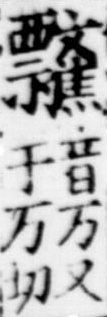
\includegraphics[height=2cm]{images/𰨘-jinpianhai.png} &
    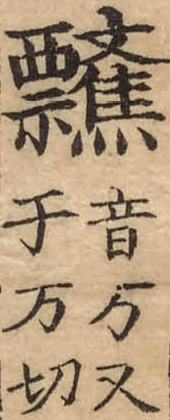
\includegraphics[height=2cm]{images/𰨘-chenghuapianhai.png} &
    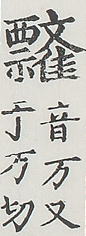
\includegraphics[height=2cm]{images/𰨘-zhengdepianhai.png} &
    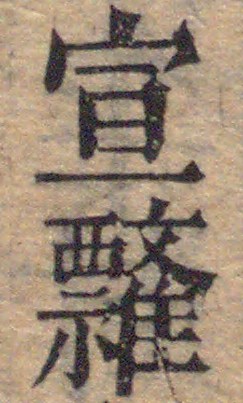
\includegraphics[height=2cm]{images/𰨘-sichuanzongzhi.png} &
    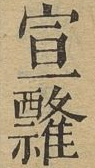
\includegraphics[height=2cm]{images/𰨘-mingshanzang.png} &
    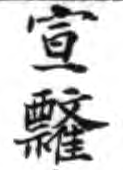
\includegraphics[height=2cm]{images/𰨘-mingshi-wan.png} &
    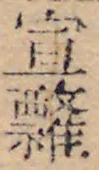
\includegraphics[height=2cm]{images/𰨘-mingshi-wang.png} &
    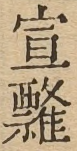
\includegraphics[height=2cm]{images/𰨘-mingshi.png} \\
    金本篇海 & 成化篇海 & 正德篇海 & 萬曆四川總志 & 名山藏 & 明史萬斯同本 & 明史稿 & 明史殿本   \\
    \entext{Jin \emph{Pianhai}} & \entext{Chenghua \emph{Pianhai}} & \entext{Zhengde \emph{Pianhai}} & \entext{Wanli \emph{Sichuan}} & \entext{\emph{Mingshan cang}} & \entext{Wan Sitong \emph{Mingshi}} & \entext{\emph{Mingshi gao}} & \entext{Palace \emph{Mingshi}} \\
    1212 & 1471 & 1515 & 1619 & 1640 & 1699 & 1723 & 1739 \\
  \end{tabularx}
\end{frame}

% ---------------------------------------------------------------------------
\begin{frame}{所據版本：正德本（續）}{The edition used: why 𰨘 points to the Zhengde edition}
  \begin{itemize}
    \item \ctu{𰨘}見於正德本篇海「西部」，正德篇海以前四聲篇海皆作「⿰票⿱文焦」之形。Unicode已編碼字形爲 U+30A18 𰨘：是王鴻緒版《明史稿》據何喬遠《名山藏》字形所改(UCV \#194)，《明史》武英殿本沿襲。
      \en{𰨘 appears under the radical 西 in the Zhengde \emph{Pianhai}; all earlier editions write ⿰票⿱文焦. The encoded form U+30A18 is the form Wang Hongxu's \emph{Mingshi gao} adapted from He Qiaoyuan's \emph{Mingshan cang} (UCV \#194), followed by the palace edition of the \emph{Ming History}.}
      %https://www.digital.archives.go.jp/img/4245626#71
      %https://commons.wikimedia.org/w/index.php?title=File%3AHarvard_drs_428231639_%E6%98%8E%E5%8F%B2_v.37.pdf&page=59
      %成化：https://guji.nlc.cn/read/book?metadataId=1398279&imageId=14337156&searchKey=%E4%BA%8E%E4%B8%87%E5%88%87
      %https://commons.wikimedia.org/w/index.php?title=File%3ANAJDA-281-0039_%E6%98%8E%E5%8F%B2%E8%97%8125.pdf&page=50
    \item 宣𰨘萬曆6年封長孫，大抵嘉靖隆慶間生，賜名當在正德本刊行之後，故取字可溯至正德本。
      \en{Xuanwan was invested as eldest grandson in 1578 and was probably born in the Jiajing or Longqing era; his name was granted after the Zhengde edition appeared, so the character can be traced to it.}
  \end{itemize}
\end{frame}

% ---------------------------------------------------------------------------
\begin{frame}{結論}{Conclusions}
  % add-ruby: skip
  \small
  \begin{enumerate}\setlength{\itemsep}{0pt}
    \item 宗室雙名：上字依字輩，下字依\textbf{五行相生}，同一世各藩五行一致
      \en{First character from the generation poem; second by the \textbf{Five-Phase generating cycle}, the same phase in every house per generation}
    \item 五行判斷依\textbf{字形部件}，不限部首：
      \en{A character's phase is judged by the \textbf{components of its form}, not just its radical:}
      \vspace{0.2em}
      {\small
        \begin{tabularx}{\linewidth}{@{}c l@{\qquad}c X@{}}
          \Mu   & \cmu{木}、\cmu{米}、\cmu{禾}       & \Jin  & \cjin{金} \\
          \Huo  & \chuo{火}、\chuo{魚}、\chuo{黑}、\chuo{光}   & \Shui & \cshui{水}、 \cshui{氵} \\
          \Tu   & \multicolumn{3}{l}{\ctu{土}、\ctu{隹}、\ctu{去}、\ctu{角}、\ctu{至}、\ctu{里}、\ctu{吉}、\ctu{赤}、\ctu{走}、\ctu{堇}} \\
      \end{tabularx}}
    \item 一字含多行部件時，可隨輩份跨行使用
      \en{A character containing components of several phases can serve different phases as the generation requires}
    \item 僻字多見於明中葉以後，取自同時代字書（正德本《四聲篇海》等）
      \en{Rare characters, mostly from the mid-Ming on, come from contemporary dictionaries (e.g.\ the Zhengde \emph{Pianhai})}
    \item 後世文獻常改作帶部首之字，甚至連字輩一同類化
      \en{Later texts often changed them to characters with the expected radical, sometimes assimilating the generation character as well}
  \end{enumerate}
\end{frame}

% ---------------------------------------------------------------------------
\begin{frame}[c]
  \centering
  \Huge Q \& A
  \vspace{1em}

  \normalsize
\end{frame}

\begin{frame}[allowframebreaks]{參考文獻}{References}
  \nocite{*}
  \printbibliography[heading=none]
\end{frame}

\end{document}
